\section{Conceitos Importantes}\label{sec:conceitos}

    Neste capítulo alguns conceitos importantes para compreender o projeto serão elaborados de forma a providenciar uma base forte para o resto do relatório. 

    \subsection{Mercado de Seguros de Londres}\label{sec:mercado-de-seguros-londres}

        Neste capítulo, far-se-á uma análise abrangente do mercado de seguros de Londres, de um ponto de vista histórico, contemporâneo e dos mecanismos intrínsecos que formam as seguradoras na capital britânica. Ao explorar a história e os funcionamentos do setor espera-se estabelecer as bases para uma análise detalhada do Projeto e como este se integra no mundo atual.

        \subsubsection{A evolução do setor de seguros de Londres}\label{secsec:a-evolucao-do-setor-de-seguros-de-londres}
    
            As origens do setor de seguros de Londres como o conhecemos hoje estendem-se por vários séculos, mas foi a partir do século \Romannum{17} com a fundação de Lloyd's e o grande fogo de Londres que se começou a formar o mercado de seguros como ainda hoje opera. 
        
            Antes deste século, um momento crítico na evolução do setor foi o caso de Gybbons v. Martin em 1537, onde o tribunal decidiu a favor do segurado em casos de ambiguidade do contrato. Aparentemente alguns \textit{underwriters} ou seguradores tinham concordado em fazer um seguro de vida para o Mr. Gybbons por um ano, e, com certeza, ele morreu uns dias antes do ano acabar. Mas os seguradores disseram que na verdade referiam-se a um ano lunar no contrato, que tinha acabado uns dias antes, claro que a Mme. Gybbons não aceitou e foi a tribunal que acabou por decidir em favor dela. 
            
            O caso estabeleceu o princípio de que qualquer incerteza na apólice seria resolvida a favor do segurado se fosse o segurador que redigisse o contrato. Esta decisão refletiu-se na indústria, causando uma solidificação do conhecimento do funcionamento e da regulação envolvendo estas matérias e contribuiu para a maturação do setor, sendo considerado um dos pilares na evolução sua evolução.  
        
            Em 1601, dois anos antes da morte da grande Rainha, um Ato do Parlamento visionava estabelecer um tribunal para ``ouvir e decidir causas decorrentes de apólices de seguro''. Embora o tribunal não fosse muito bem-sucedido, demonstrou que os princípios do seguro eram conhecidos entre aqueles que com eles lidavam.
            
            Edward Lloyd, nascido por volta de 1648, uma figura não diretamente envolvida em seguros, mas dono de uma cafetaria, desempenhou um papel fundamental no desenvolvimento do setor. Disponibilizou cabines na sua cafetaria para empresários dispostos a acartar uma parte do risco mediante uma taxa, e foi onde a tradição de '\textit{writing under}' começou. Os seguradores assinavam nas apólices debaixo do risco, surgindo assim o termo ``\textit{Underwriter}''.
        
            Em 1666, houve o Grande Incêndio de Londres, que devastou grande parte da cidade e consumindo inúmeras construções históricas, impulsionando mudanças no setor de seguros como a criação da primeira companhia de seguros de incêndio, The Sun. Isto incitou a mais movimento na cafetaria de Lloyd cujo negócio continuou a criar as bases para seguros marítimos e pagando quando necessário da parte dos seguradores como foi o caso, por exemplo, do naufrágio do Titanic\cite{lloyd-titanic}. A consistência de Lloyd's em pagar as perdas permanece consistente há mais de três séculos, sendo uma referência sólida na indústria de seguros\cite{lloyds-and-the-great-fire-of-london-propertycasualty360}.

        \subsubsection{O setor de seguros de Londres contemporâneo}\label{sec:o-setor-de-seguros-de-londres-contemporaneo}
    
            Em 2013, o setor de seguros representou impressionantes 20\% do Produto Interno Bruto (PIB) da cidade e 8\% do PIB de Londres. Esta significativa contribuição demonstra a importância económica do setor de seguros no contexto da capital britânica.
            
            Adicionalmente, o mercado londrino destaca-se ao segurar ativos valiosos e únicos. Exemplos notáveis incluem a cobertura para as pernas do renomeado jogador de futebol Cristiano Ronaldo e a voz única de Bruce Springsteen. Esta capacidade de segurar riscos especializados sublinha a flexibilidade e abrangência do mercado de seguros de Londres, atendendo às necessidades específicas de indivíduos e personalidades públicas.
        
            % 1 bilião deste lado do oceano é um milhão vezes um milhão
        
            % What Is an Insurance Premium? An insurance premium is the amount of money an individual or business pays for an insurance policy.
            % Gross written premium is a term that may refer to the total amount of premiums collected by an insurance company during a given period before any discounts or refunds are taken into account.
                
            Como visto na Figura \ref{fig:biggest-insurance-markets}, o mercado de seguros de Londres assume a primeira posição global, sendo o maior centro mundial de riscos comerciais e especializados. Em 2013, o mercado londrino controlou mais de £60 bilhões em ``GWP'', refere-se à quantidade de dinheiro paga à seguradora, fazendo deste o maior mercado mundial neste setor, superando significativamente a concorrência, com o segundo maior, o mercado de Bermuda, apresentando um tamanho de mercado de £25 bilhões em ``GWP''\cite{the-competitive-position-of-the-london-insurance-market,how-the-london-insurance-market-works}. % parencites
        
            \begin{figure}[H]
                \centering
                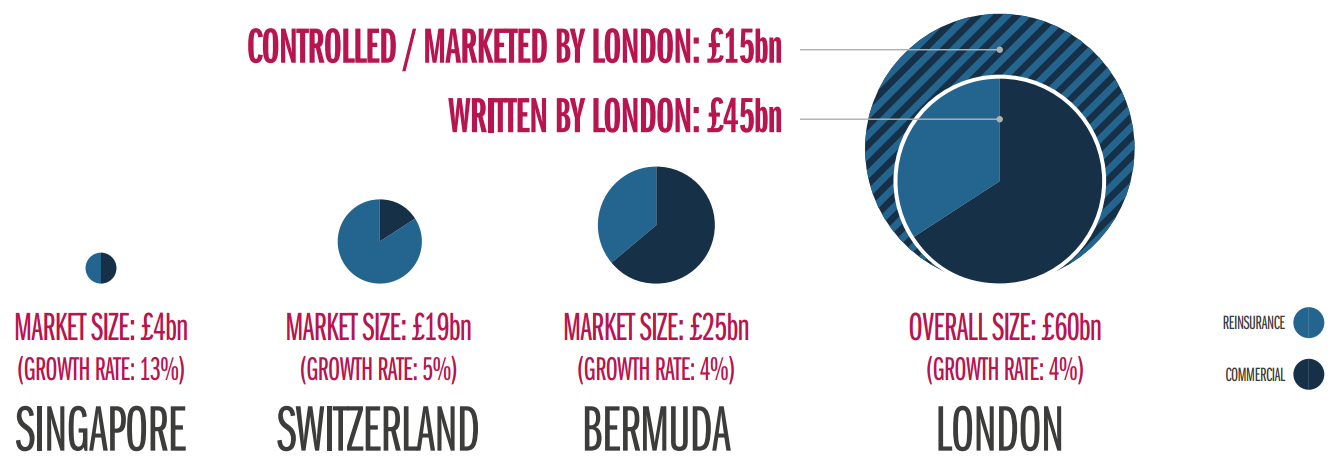
\includegraphics[width=\textwidth]{imgs/Biggest_Insurance_Markets.png}
                    \caption{Maiores mercados de seguros - 2013}\label{fig:biggest-insurance-markets}
                    \source{\cite{the-competitive-position-of-the-london-insurance-market}}
            \end{figure}

        \subsubsection{Funcionamento e Terminologia de seguradoras}\label{secsec:mercado-de-londres-tradicional}

            O mercado de Londres é um campo onde jogam muitas empresas ou sindicatos que serão representadas pelos \textit{underwriters}. É normal subscreverem vários \textit{underwriters} para dividirem o risco entre si.

            O processo de emissão de seguros no século \Romannum{17} mantém-se no século \Romannum{21}: \\
            Aqueles que procuram segurar-se dirigem-se a um \textit{broker} e explicam o seu risco de forma detalhada, a qualidade e preço das ofertas depende da quantidade das informações fornecidas. O \textit{broker}, de seguida, vai ao encontro de \textit{underwriters} que representam um sindicato de um investidor, procurando os que podem oferecer melhores taxas consoante o risco em causa. O \textit{underwriter} pode dizer, por exemplo, ``Aceito 8\% a 2 por 250'', nesta situação este \textit{underwriter} cobre 8\% do risco, a uma taxa de 2 por 250 unidades monetárias. Desdobrando a proposta em mais detalhe:
            \begin{itemize}
                % \item Uma rate de 2 por 250
                \item Uma taxa de 2 por 250 indica que se o segurado tem 250€ de propriedade segurada exposta a risco, o segurado teria que pagar um prémio de 2€, ou seja, teria que pagar pelo seguro 2€ anualmente (ou mensalmente conforme estipulado). Mas isto apenas se estiver segurado a 100\%;
                \item Aceita 8\% do risco, ou seja, cobre apenas 8\% do valor caso o seguro se ative e recebe apenas 8\% do prémio.
            \end{itemize}
            De seguida o \textit{broker} dirigia-se a outros \textit{underwriters}, já com a taxa estipulada e tenta segurar o máximo de risco possível. Por vezes 100\% do risco é subscrito mas geralmente menos é segurado, e o proprietário ou comerciante é co-segurado para o resto, ou seja, é responsável pelo pagamento do restante\cite{rate-making,lloyds-and-the-great-fire-of-london-propertycasualty360}.

            % Titanic
            É frequente para projetos de alto capital serem segurados por bastantes \textit{underwriters} dividindo o risco entre eles, segundo os documentos de seguros do Titanic, por exemplo, o navio encontrava-se segurado por mais de 70 \textit{underwriters} diferentes\cite{titanic2,titanic}, como visto na Figura \ref{fig:titanic-placement-slip}.

            \begin{figure}[H]
                \centering
                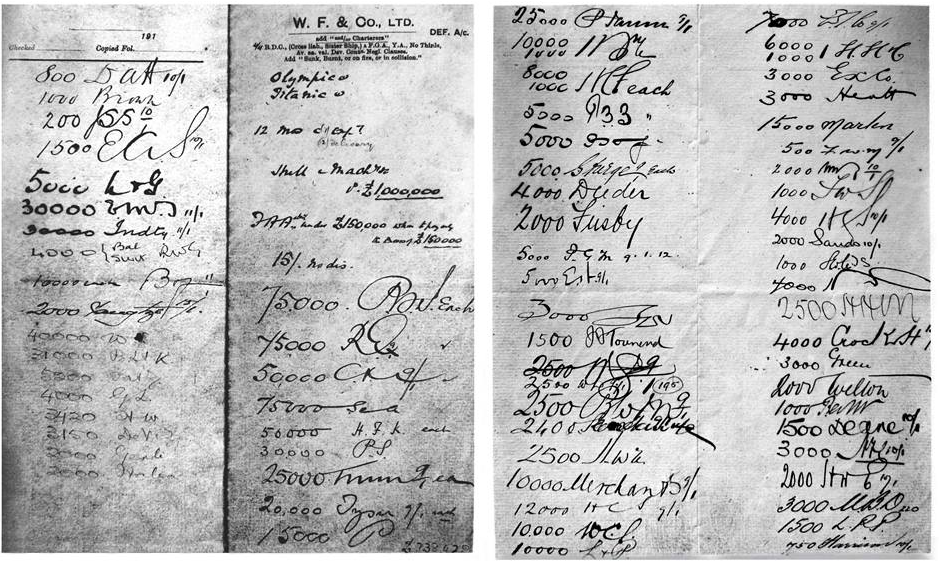
\includegraphics[width=\textwidth]{imgs/Titanic-Placement-Slip1.png}
                    \caption{Titanic Placement Slip — 2013}\label{fig:titanic-placement-slip}
                    \source{\cite{titanic}}
            \end{figure}

            % percebendo o que é "Aceito 8\% a 2 por 250"
            % https://www.businessinsider.com/personal-finance/what-is-underwriting
            % Underwriting helps set rates for loans, premiums for insurance policies, and the cost of risk in securities markets.

            % video que demonstra como underwriters são basicamente gajos que apostam no stock market: https://www.youtube.com/watch?v=QmJObCXq_Hk
        
            % https://www.irmi.com/term/insurance-definitions/placement-slips#:~:text=Placement%20slips%20are%20a%20general,transaction%E2%80%94not%20a%20binding%20contract.
            %Placement slips are a general understanding of the terms and conditions of a reinsurance transaction—not a binding contract.

            Com o processo geral estipulado pode-se agora detalhar as semânticas dos termos usados:

            \begin{itemize}
                \item \textbf{Underwriter:} O \textit{underwriter}, ou subscritor, é o profissional ou entidade responsável por assumir o risco do seguro. Avalia o risco, discute e estabelece os termos da cobertura e define a taxa e o prémio;
                
                \item \textbf{Broker:} O \textit{broker}, ou corretor, atua como intermediário entre o segurado e os \textit{underwriters}. Ele ajuda o segurado a compreender as suas necessidades, negocia com os \textit{underwriters} em nome dele e facilita o processo de subscrição;
                
                \item \textbf{Syndicate:} Um \textit{syndicate}, ou sindicato, refere-se a um grupo de \textit{underwriters} que se unem para assumir um determinado risco. Cada membro do sindicato contribui com uma parte da subscrição;
                
                \item \textbf{Placement Slip:} É um documento preliminar que resume os detalhes essenciais de um contrato de seguro. Inclui informações sobre o risco, cobertura, termos e \textit{underwriters} envolvidos;
                
                \item \textbf{Endorsements:} Referem-se a alterações feitas a uma apólice de seguro existente. Podem incluir a adição, remoção ou modificação de coberturas, condições ou termos do contrato. Estes são utilizados regularmente para ajustar a apólice conforme as necessidades do segurado;
    
                \item \textbf{Sign \& Close:} A etapa de ``Sign and Close'' refere-se ao processo de finalização de um contrato de seguro. Envolve a assinatura formal do contrato pelos participantes relevantes, confirmando a aceitação dos termos acordados. Este passo conclui o processo de subscrição e torna o contrato efetivo.

            \end{itemize}

            Este processo é comparável ao investimento numa empresa, \textit{underwriters} podem envolver-se com empresas de banca ou de seguros com títulos de valor variável de empresas (``\textit{securities}''). Da mesma forma que se pode lucrar ao investir num setor ou empresa, os \textit{underwriters} acartam risco para gerar lucro\cite{underwriting-insurance-loans-ipos-etc-explained-in-one-minute}.
    
            % To-Do: Podes falar de como funciona na plataforma:  Master facilities, placements, e a hierarquia de users e comapnhias etc

    \subsection{Desenvolvimento \textit{Low-Code}}\label{sec:low-code}

        Esta secção fornece uma resposta às questões de pesquisa sobre a definição do desenvolvimento \textit{low-code}, o seu ciclo de vida, bem como características e especificidades relacionadas.

        \subsubsection{Definição de Desenvolvimento \textit{Low-Code}}\label{secsec:defining_low-code}

            O termo ``\textit{low-code}'' surgiu em 2014 num artigo da \textit{Forrester Research} intitulado ``New Development Platforms Emerge For Customer-Facing Applications'' de Richardson C. \cite{bock2021lowcode,sanchis2020lowcode,bucaioni2022modelling,diruscio2022lowcode}, e desde a altura que tem ganhado tração e se solidificado como um campo da informática, num artigo de Alamin, \cite{alamin2021empirical} o desenvolvimento \textit{low-code} é definido como um paradigma que prioriza o mínimo de programação no processo, isto através de programação visual com interface gráfica e \textit{design} orientado por modelos. Noutras definições é também definido como um processo que envolve um esforço de programação mínimo com funcionalidades como \textit{drag-and-drop}\footnote{um paradigma de interface gráfica onde o utilizador pode selecionar elementos digitais, como ícones ou arquivos, movendo-os de um local para outro simplesmente ao clicar, manter o botão pressionado e soltando no destino desejado.} e desenvolvimento acessível a programadores não profissionais\cite{rokis2023exploring}.

        \subsubsection{Benefícios de Desenvolvimento \textit{Low-Code}}\label{secsec:beneficios_low-code}

            O desenvolvimento \textit{low-code} oferece diversas vantagens estratégicas, conforme destacado na lista abaixo. Ao acelerar o ciclo de desenvolvimento e envolver programadores menos especializados, esta abordagem responde eficientemente à escassez de profissionais especializados, permitindo uma entrega mais rápida de aplicações. A redução de custos é alcançada através da eficácia no desenvolvimento, otimização de recursos e diminuição dos custos de manutenção. Esta prática também aumenta a capacidade de resposta às exigências do mercado e dos negócios, adaptando-se rapidamente a situações dinâmicas e cumprindo prazos apertados, minimizando o esforço de manutenção e promovendo uma colaboração mais eficaz entre as equipas de desenvolvimento e as empresas, fomentando um ambiente propício à inovação digital\cite{rokis2023exploring,yan2021impacts}.

            \begin{itemize}
                \item \textbf{Aceleração do ciclo de desenvolvimento:} Aproveita as funcionalidades da plataforma, minimizando a programação manual e incorporando um desenvolvimento visual de aplicações;
                \item \textbf{Envolvimento de programadores cidadãos:} Aborda a escassez de programadores especializados, contribuindo para uma entrega mais rápida de aplicações;
                \item \textbf{Redução de custos:} Alcançada através da rapidez do desenvolvimento, utilização eficiente de recursos e diminuição dos custos de manutenção;
                \item \textbf{Aumento da capacidade de resposta às exigências do mercado e dos negócios:} Adapta-se rapidamente a situações dinâmicas e cumpre prazos apertados;
                \item \textbf{Diminuição do esforço de manutenção:} Minimiza erros e problemas relacionados à integração, permitindo a contínua manutenção menos exigente;
                \item \textbf{Melhor colaboração entre equipas de desenvolvimento e empresas:} Facilitada por modelos visuais e colaboração frequente ao longo do ciclo de desenvolvimento;
                \item \textbf{Promoção da inovação digital:} Fomenta uma cultura de aprendizagem e experimentação;
                \item \textbf{Mitigação dos riscos de \textit{shadow IT}\footnote{programas e sistemas de TI utilizados sem a aprovação do departamento de TI da organização, apresentando, portanto, riscos de segurança, integridade dos dados e outros.}:} Através de ferramentas administradas pela organização a profissionais não pertencentes à área 
                de TI, reduzindo soluções não autorizadas de TI e os riscos associados\cite{rokis2023exploring}.
            \end{itemize}

            Em 2019 a OutSystems analisou o estado da área de desenvolvimento \textit{low-code}, revelando as principais razões que impulsionam empresas a adotar estas metodologias como é possível observar na Figura \ref{fig:reasons_to_use_low-code}, estas incluem: a aceleração da inovação e transformação digital, o aumento da capacidade de resposta às exigências do negócio, a redução da dependência de habilidades técnicas de difícil contratação, a mitigação de despesas devido a tecnologias obsoletas, a proteção contra a rápida evolução tecnológica, e permitir programadores cidadãos aprimorarem processos internos.
    
            \begin{figure}[htbp]
                \centering
                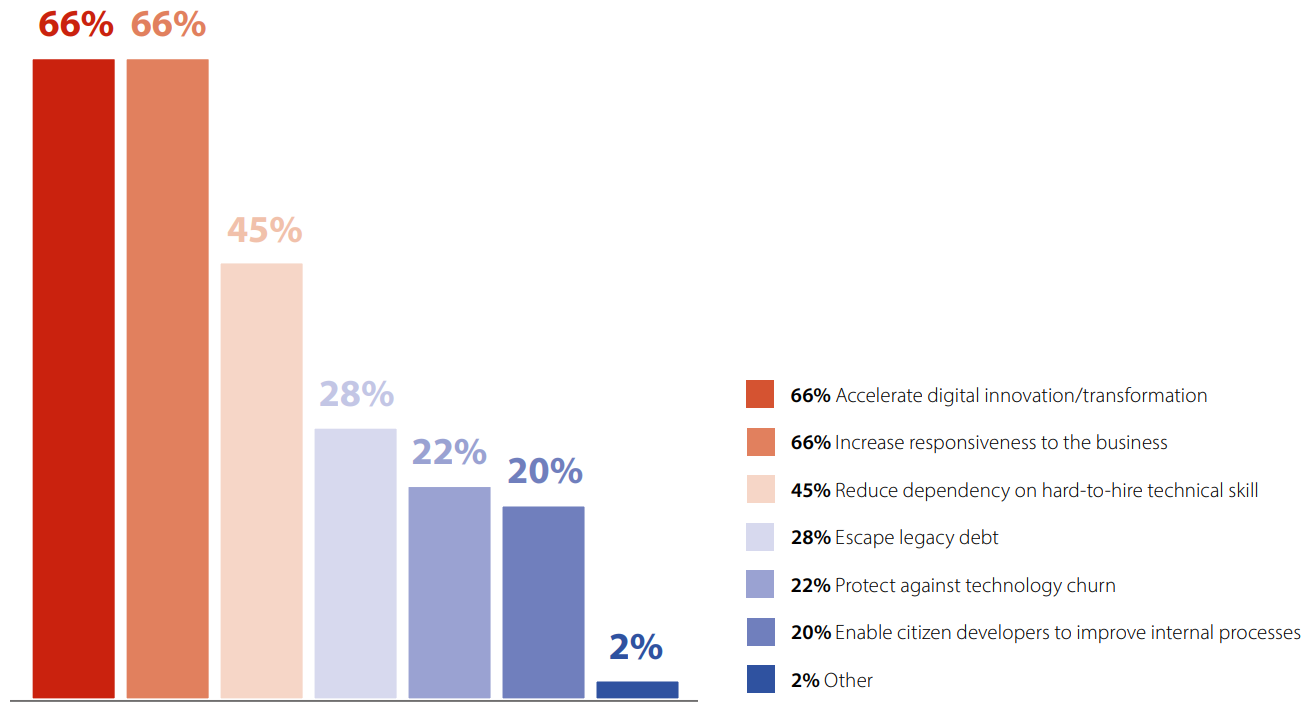
\includegraphics[width=\textwidth]{imgs/reasons_to_use_low-code.png}
                    \caption{Maiores razões para usar \textit{low-code}}\label{fig:reasons_to_use_low-code}
                    \source{\cite{state-of-lowcode-outsystems}}
            \end{figure}

        \subsubsection{Limitações de Desenvolvimento \textit{Low-Code}}\label{secsec:limitacoes_low-code}

            A OutSystems identificou no seu estudo ``The State of Application Development'' de 2019, segundo os participantes os três desafios que mais dificultam a entrega de aplicações móveis e de web são:
            \begin{itemize}
                \item Integração com sistemas obsoletos ou ultrapassados;
                \item Requerimentos não bem definidos e inconstantes;
                \item Tempo necessário para testar.
            \end{itemize}
                
            Identificando também as maiores causas de retardam a entrega destas aplicações, como visto na Figura \ref{fig:atraso_app_low_code}, sendo estas, a Integração de sistemas legados/APIs ausentes ou que necessitam de melhorias, Requisitos difusos/em constante mudança, Testes/Garantia de Qualidade, Proteção e teste de penetração em segurança, Preocupações com privacidade de dados, Falta de habilidades técnicas de desenvolvimento, \textit{Design} UX/UI (incluindo \textit{design} responsivo), Implantação/coordenação com operações de TI\cite{state-of-lowcode-outsystems}.
                
            \begin{figure}[htbp]
                \centering
                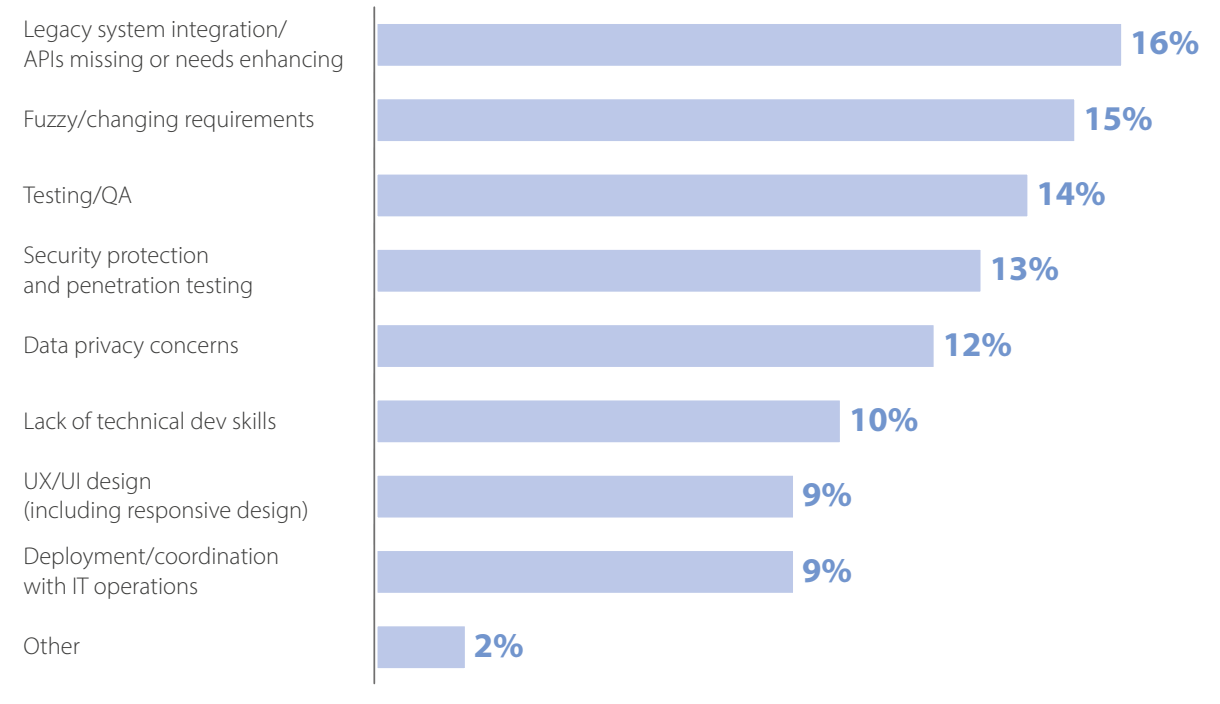
\includegraphics[width=\textwidth]{imgs/causas_espera_na_entrega_aplicacoes_low_code.png}
                    \caption{Maiores causas de atrasos na entrega de aplicações \textit{low-code}}\label{fig:atraso_app_low_code}
                    \source{\cite{state-of-lowcode-outsystems}}
            \end{figure}
            
            Segundo o artigo ``The Impacts of Low/No-Code Development on Digital Transformation and Software Development'' do autor Zhaohang Yan podem ser identificadas estas limitações no método:

            \begin{enumerate}
                \item \textbf{Limitação na Customização/Flexibilidade:}  Estas plataformas têm pré-implementações fixas em muitas áreas e casos, tornando-as menos customizáveis sacrificando flexibilidade. Programar funcionalidades customizáveis específicas é uma opção, mas pode ser difícil e moroso, podendo não ser o método ideal para aplicações que precisem de ser altamente customizáveis com um nível de complexidade mais elevado.
            
                \item \textbf{Limitação na Scalabilidade:} Muitas destas plataformas focam num processo célere na produção e entrega de aplicações de pequena a média escala, sendo uma ferramenta menos testada para aplicações de grande escala.
            
                \item \textbf{Preocupações de Segurança:} A utilização de plataformas \textit{low-code} implica a inteira dependência da segurança da plataforma em uso. Organizações dependentes destas plataformas enfrentam riscos, uma vez que a segurança dos dados não está totalmente sob o seu controle. Se, por exemplo, os fornecedores da plataforma encerrarem as operações, as atualizações de segurança contínuas tornam-se incertas, deixando as organizações incapazes de lidar com novas vulnerabilidades.

                \item \textbf{\textit{Vendor lock-in}:} Refere-se à dependência de um cliente em relação a um fornecedor, e à sua capacidade de mudar para outro. No contexto das plataformas \textit{low-code}, à medida que investem mais num fornecedor específico, o processo de mudança torna-se mais dispendioso e complexo e difícil\cite{yan2021impacts}.
            \end{enumerate} 

            Em suma, existem vários detalhes específicos ao desenvolvimento \textit{low-code}, sendo importante analisar as vantagens expostas e as desvantagens identificadas e os seus pesos na implementação num dado projeto.

    \subsection{Terminologia do Projeto}\label{sec:terminologia_do_projeto}
        
        Existem vários conceitos que serão frequentemente utilizados ao longo deste relatório e são frequentemente usados no contexto de trabalho, esta secção servirá para estabelecer bem os seguintes conceitos:

        \begin{itemize}
            \item \textbf{User Stories:} As \textit{User Stories} (Histórias de Utilizador) são descrições detalhadas de funcionalidades do sistema, frequentemente utilizadas para comunicação entre os interessados e para orientar o desenvolvimento de software. Elas são a base para o desenvolvimento na plataforma;

            \item \textbf{Defects}\label{bulletlist:defects}: Uma incongruência identificada entre o funcionamento do programa e as USs (User Stories) definidas. São identificados com uma prioridade e registadas na Jira como descrito na Secção \ref{secsec:jira};
            
            \item \textbf{Incidentes}\label{bulletlist:incidentes}: Problemas submetidos por utilizadores da aplicação através da plataforma ServiceNow [\ref{sec:service-now}], o utilizador pode marcar a submissão de duas formas:
            \begin{itemize}
                \item \textbf{Request}: O utilizador coloca esta \textit{label} quando não tem a certeza se o problema está na forma de utilização ou de facto na plataforma;
                \item \textbf{Incidente}: Se o utilizador está confiante que o problema com que se depara é de facto um problema da plataforma, marca desta forma.
            \end{itemize}

            \item \textbf{GAP}: Caso específico em que a implementação está de acordo com a \textit{user story}, mas a esta não contempla uma situação que se precisava de ter em conta.
            
            Por exemplo: Se a \textit{user story} for ``Efetuar um programa que conte de um a cinco'', e o programa conte da seguinte forma: ``1, 2, 3, 4, 5'', mas se descubra através de testes ou interações com utilizadores e confirmando com um BA ou alguém mais acima na hierarquia que esteja familiarizado com o que a aplicação tem que fazer, que a aplicação teria que contar também decimais desta forma: ``1.1, 1.2, 1.3...'', então, como não estava bem explícito na US, considera-se um GAP.
            
            É por isso que antes de reportar um novo \textit{defect}, é geralmente necessário confirmar que o comportamento que acontece não está contemplado numa \textit{user story}, porque se estiver, será um GAP. Neste caso a \textit{user story} terá que ser revista, e a empresa cliente terá possivelmente que pagar por outra US, visto que o pagamento se faz por USs;
            
            %GAP - Quando falta alguma coisa na user storie e se reflete no desenvolvimento
            %- Por exemplo, caso especifico em que UW não recebia notificação, mas aquele.
            \item \textbf{Stamps:} Num contexto de lógica de seguradoras, os Stamps representam a aprovação formal de um \textit{underwriter} para assumir um risco específico. Cada \textit{underwriters} coloca seu carimbo no \textit{Placement Slip} como uma indicação da sua subscrição no risco.

            No contexto da plataforma, stamps são carimbos associados a uma organização cujos UWs pertencentes podem usar. Após a definição dos detalhes de um contrato e antes do envio da submissão aos UWs pertencentes, são atribuídos \textit{roles}, estes \textit{roles} são escolhidos consoante o stamp de cada UW. Podendo um UW não ter nenhum \textit{role};
                
            % todo confirmar que é isso que quer dizer, e mudar também nas abreviações e noutro sítio se for pra mudar
            \item \textbf{Mutual Responsibility Contract(MRC):} O MRC, é um documento obrigatório a todos os contratos na plataforma que contém detalhes sobre o acordo que possam não estar contemplados na plataforma como informações de cobertura de uma apólice de seguro ou detalhes sobre o risco coberto, ou as condições e termos do contrato;

            \item \textbf{Endorsements:} Como explicado na Secção \ref{secsec:mercado-de-londres-tradicional}, referem-se a alterações feitas a um contrato, na plataforma existem os seguintes tipos de endorsement:
            \begin{enumerate}
                \item Annual Resigning Statement;
                \item Cancellation;
                \item Decrease Cover;
                \item Increase Cover;
                \item Mid-Term Broker Change;
                \item Other Change to Cover;
                \item Reinstatement Provision;
                \item Tax Schedule;
                \item Mid Term Market Change (o único \textit{endorsement} que requer um \textit{Sign \& Close}).
            \end{enumerate}
            A termos de lógica de negócio a única diferença está entre o Mid Term Market Change e os restantes, devido ao seu requisito de ser feito num contrato \textit{Signed and Closed};

            \item \textbf{Corrections:} Correções são modificações realizadas para retificar erros ou informações incorretas em documentos relacionados ao seguro. Estas podem incluir ajustes nas apólices, documentos contratuais ou registos relacionados à subscrição. Na plataforma existem três tipos de \textit{corrections}:
            \begin{itemize}

                 \item \textbf{Cancel Contract:}
                 A ação ``Cancel Contract'' permite ao \textit{broker} cancelar completamente um \textit{placement} de forma irreversível. A aceitação por parte da seguradora de um pedido de cancelamento reduz a linha escrita para zero e altera o estado do contrato para Cancelado. Uma vez concluído o cancelamento, é possível reutilizar o UMR. 
                 
                 No caso de cancelamento de uma \textit{master facility}, as partes não acordadas serão canceladas assim que o líder da \textit{facility} aceitar o cancelamento. Um pedido de cancelamento para qualquer \textit{declaration} já vinculada que utilize a \textit{facility} será acionado simultaneamente;
                 
                 \item \textbf{Cancel and Replace:}
                 A ação ``Cancel and Replace'' está disponível ao longo do processo de \textit{Firm Order}. Permite ao \textit{broker} substituir um contrato cancelando o original simultaneamente de forma irreversível. A aceitação por parte da seguradora de uma ressubmissão vincula a linha escrita ao novo contrato, reduzindo a linha no contrato anterior para zero e alterando o estado para Cancelado. Não é possível assinar e fechar até que todas as submissões originais sejam canceladas e todas as ressubmissões sejam aceites;
                 
                 \item \textbf{Panel Change:}
                 A ação ``Panel Change'' está disponível ao longo do processo de \textit{Firm Order}. Permite ao \textit{broker} fazer alterações nos detalhes da linha dos participantes no contrato. Incluindo em painéis de \textit{facilities}, desde que o líder da \textit{facility} não seja um Slip, Lloyds, XIS ou LIC Lead no \textit{placement}. Detalhes da linha que podem ser alterados incluem linha escrita e stamp. A ação é irreversível, sendo necessário responder a todos os pedidos de ``Panel Change'' antes de assinar e fechar.
            \end{itemize}           

            \item \textbf{Master Facilities:} Master Facilities ou Facilities referem-se a um conjunto de seguradoras que se juntaram e aceitaram fazer parte da \textit{facility}, esta que depois pode ser adicionada como painel conjunto a um contrato;

            \item \textbf{Declarations e Open Market Contracts:} \textit{Declarations} e contratos de mercado aberto referem-se a contratos que utilizam painéis de \textit{facilities} ou não. As \textit{declarations} são contratos que envolvem uma ou mais \textit{facilities}, já contratos de mercado aberto envolvem apenas UW individuais;
            
            \item \textbf{Off-platform Underwriters:} \textit{Underwriters} fora da plataforma são profissionais que assumem riscos de seguro, mas que não utilizam diretamente a plataforma para a subscrição. A interação eficaz com esses \textit{underwriters} é simulada na plataforma por um UW \textit{off-platform} cujas respostas ao contrato são controladas pelo \textit{broker}, desta forma este deve alinhar com estes UWs fora da plataforma e consoante o decidido, colocar a resposta por eles na plataforma;
            
            \item \textbf{Archive Placements:} Refere-se ao armazenamento organizado de registos e documentos relacionados a colocações de seguros já fechados. É muito usado na transferência de dados de uma plataforma antiga;
            
            \item \textbf{Placements:} Referem-se a uma estrutura que pode conter vários contratos. É obrigatório um contrato se encontrar sempre dentro de um \textit{placement};
            
            \item \textbf{Firm Order:} É o processo vinculativo executado pelo \textit{broker} que manda os pedidos de aceitação do cancelamento ou do endorsement ou das linhas do contrato para os UWs. Pelo que mandar uma \textit{firm order} será mandar o pedido em contexto para os UWs apropriados;
            
            \item \textbf{Retrofit:} É a passagem de código de um ambiente mais avançado, ou seja, mais próximo do ambiente de produção, para um ambiente de mais baixo nível, como por exemplo um dos ambientes de desenvolvimento, isto pode ser necessário, por exemplo, se um \textit{defect} teve que ser resolvido num ambiente mais alto de forma a que a sua resolução chegue mais rápidamente a produção, neste caso ter-se-ía que trazer este código para os ambientes mais baixos também, a este processo chama-se retrofit, refira à Secção \ref{secsec:versionamento} para mais informação sobre ambientes;
            
            \item \textbf{Cancel Line:} Cancelar uma linha representa a anulação de uma linha específica num contrato de seguro, ou seja de um UW ou de uma \textit{facility}. Após os relevantes terem aceite, se não tiverem nenhum \textit{role} gerado pelos seus stamps, o \textit{broker} pode lhes fazer um cancel line, que irá mandar um pedido para se retirarem;
            
            \item \textbf{Withdraw:} A ação de withdraw está disponível depois de fazer uma submissão para um UW, mas antes deste aceitar. Ao fazer \textit{withdraw}, o UW não poderá mais aceitar o pedido;

            \item \textbf{Business Analysts (BA)}: Os \textit{Business Analysts} analisam e compreendem os processos e funcionamento de negócios, identificando oportunidades de melhoria, desempenhando tarefas como análise de dados, comunicação com clientes, documentação de processos, testes e validações. 

            Na prática, os BA's são generalistas da equipa que têm uma boa noção de como a aplicação se deve comportar e a quem se recorre em caso de dúvida.
           
        \end{itemize}